\section{Clustering di punti}
\label{sec:clustering_di_punti}

Un altro problema abbastanza comune nell'elaborazione di dati geometrici è quello di raggruppare un insieme di punti in sottoinsiemi (\emph{cluster}) coerenti, in base alla loro posizione. A differenza della ricerca di prossimità, che risponde a interrogazioni puntuali, il clustering spaziale ha l'obiettivo di partizionare l'intero insieme di dati, individuando automaticamente quali punti appartengono allo stesso oggetto e quali, invece, sono isolati o rappresentano rumore.

La categoria degli algoritmi più adatta è quella degli \emph{density-based}, in particolare \textbf{DBSCAN} (\emph{Density-Based Spatial Clustering of Applications with Noise}), introdotto da Ester et al. \cite{ester1996dbscan}. A differenza di algoritmi come \emph{k-means}, che richiedono di specificare a priori il numero di cluster e tendono a produrre cluster di forma convessa, DBSCAN definisce i cluster come regioni di spazio ad alta densità di punti separate da regioni a bassa densità, ed è quindi in grado di identificare cluster di forma arbitraria e di isolare automaticamente i punti isolati come rumore \cite{builtin_dbscan}.

\subsection{L'algoritmo DBSCAN}

Prendo come riferimento l'articolo di Okan Yenigün \cite{builtin_dbscan}. Per capire come funziona l'algoritmo DBSCAN consideriamo il seguente esempio:
\begin{figure}[htbp]
	\centering
	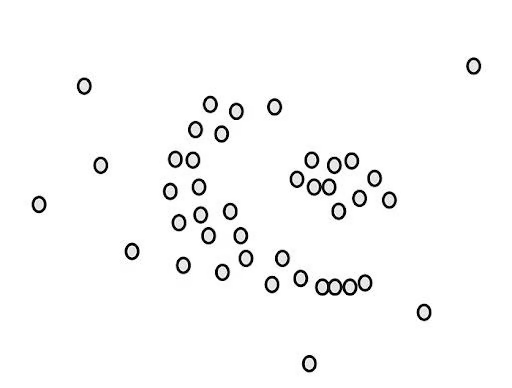
\includegraphics[width=0.5\textwidth]{figures/2_background_teorico/1_dbscan.png}
\end{figure}
 
 L'obbiettivo è di raggruppare questi punti in gruppi (cluster). Prendiamo inizialmente un punto da cui partire e disegnamo un cerchio attorno:
 \begin{figure}[htbp]
 	\centering
 	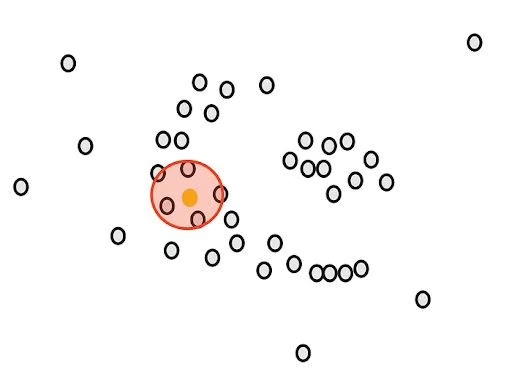
\includegraphics[width=0.5\textwidth]{figures/2_background_teorico/2_dbscan.png}
 \end{figure}
 
 Il raggio $\epsilon$ del cerchio è il primo parametro da determinare. Dopodiché contiamo quanti punti si trovano all'interno del cerchio e vediamo che ci sono esattamente 5 punti di prossimità.
 
 Adesso dobbiamo determinare un altro parametro, ovvero il numero minimo $m$ di punti. Un punto si dice essere un "core point" se è vicino almento a $m$ punti. Se consiriamo $m=3$, allora i seguenti punti evidenziati in viola sono core point, mentre il punto in giallo no.
\begin{figure}[htbp]
	\centering
	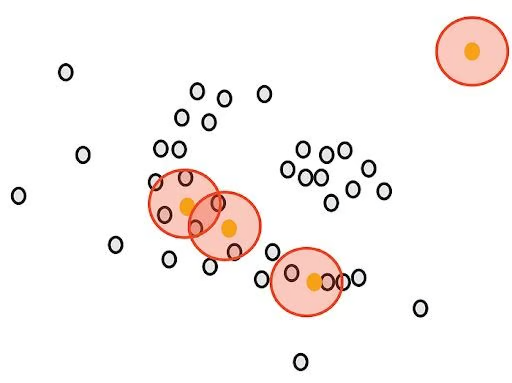
\includegraphics[width=0.5\textwidth]{figures/2_background_teorico/3_dbscan.png}
\end{figure}

 Dopo, selezioniamo a caso un core point e lo assegniamo come primo punto nel nostro primo cluster. I punti che si trovano vicino al core point vengono considerati dentro al cluster.
\begin{figure}[htbp]
	\centering
	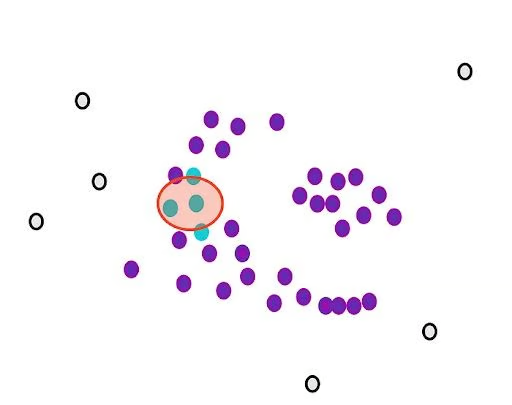
\includegraphics[width=0.5\textwidth]{figures/2_background_teorico/4_dbscan.png}
\end{figure}

 Ripetiamo il procedimento anche per gli altri punti vicini e ci fermiamo quando non possiamo più assegnare più assegnare core points al primo cluster. 
\begin{figure}[htbp]
	\centering
	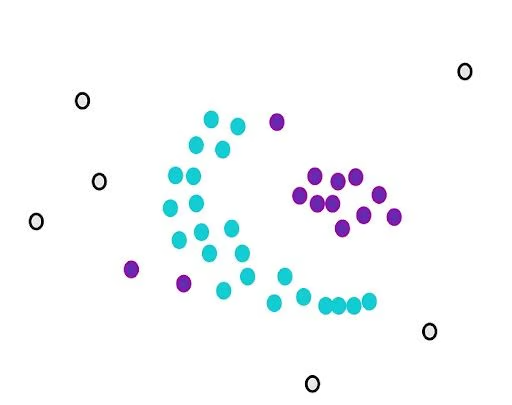
\includegraphics[width=0.5\textwidth]{figures/2_background_teorico/5_dbscan.png}
\end{figure}
\newpage
 
 Ci sono dei punti che sono vicini al primo cluster che però non sono dei core points. Deisegnamo i cerchi anche su questi punti e vediamo se rientrano nel cluster. Questi punti sono i punti di frontiera (o anomalie).
 \begin{figure}[htbp]
 	\centering
 	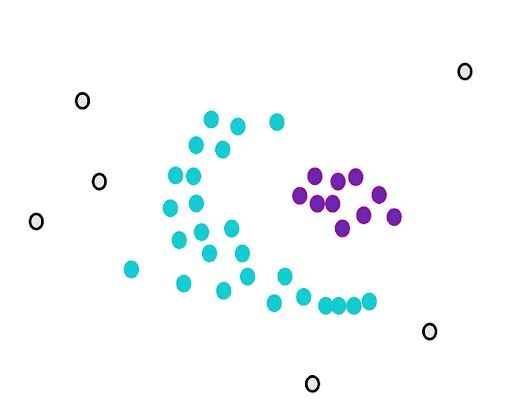
\includegraphics[width=0.5\textwidth]{figures/2_background_teorico/6_dbscan.png}
 \end{figure}

Sono rimasti altri core points che non sono ancora stati assegnati. Ne selezioniamo uno a caso e ripetiamo il procedimento.
 \begin{figure}[htbp]
	\centering
	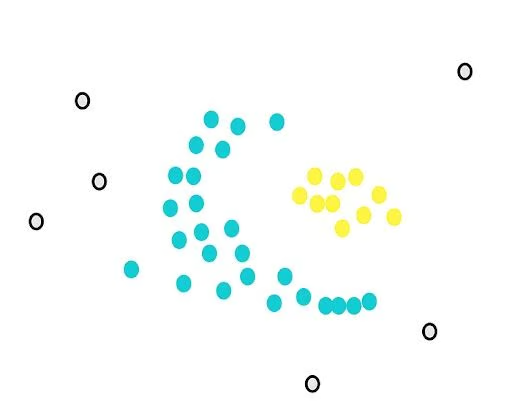
\includegraphics[width=0.5\textwidth]{figures/2_background_teorico/7_dbscan.png}
\end{figure}
\newpage

DBSCAN è un algoritmo sequenziale, è quindi importante notare che i punti non core verranno assegnati al primo cluster che soddisfa il requisito di vicinanza.

\subsection{Scelta dei parametri}

La qualità del risultato prodotto da DBSCAN dipende dalla scelta dei due parametri $\epsilon$ e $m$. Un valore di $\epsilon$ troppo grande tende a far collassare cluster distinti in un unico cluster; al contrario, un valore troppo piccolo produce una frammentazione eccessiva. Analogamente, $m$ regola la densità minima richiesta per considerare una regione un cluster: valori più alti producono cluster più densi e robusti al rumore, ma rischiano di scartare cluster legittimi composti da pochi punti.